\documentclass[11pt]{article}
\usepackage[margin=1in]{geometry}
\usepackage{amssymb,amsfonts,amsmath,amsthm,amscd,dsfont,mathrsfs,bbold}
\usepackage{blkarray}
\usepackage{graphicx,float,psfrag,epsfig,color}
\usepackage{microtype}
\usepackage[pdftex,pagebackref=true,colorlinks]{hyperref}
\usepackage{tikz}
\usepackage{natbib}

\usepackage{bm}
\usetikzlibrary{positioning}
\tikzset{main node/.style={circle,fill=white!20,draw,minimum size=1cm,inner sep=0pt},}
\hypersetup{linkcolor=[rgb]{.7,0,0}}
\hypersetup{citecolor=[rgb]{0,.7,0}}
\hypersetup{urlcolor=[rgb]{.7,0,.7}}

\newcommand{\remove}[1]{}
\setlength{\topmargin}{0.2in} \setlength{\headheight}{0in}
\setlength{\headsep}{0in} \setlength{\textheight}{8.7in}
\setlength{\topsep}{0in} \setlength{\itemsep}{0in}
\parskip=0.060in

\textwidth=6.6in \oddsidemargin=0truecm \evensidemargin=0truecm



\hbadness=10000 \vbadness=10000

\setlength{\oddsidemargin}{.25in}
\setlength{\evensidemargin}{.25in} \setlength{\textwidth}{6in}
\setlength{\topmargin}{-0.4in} \setlength{\textheight}{8.5in}

\newcommand{\details}[8]{
	\renewcommand{\thepage}{#1-\arabic{page}}
	\noindent
	\begin{center}
		\framebox{
			\vbox{
				\hbox to 5.78in { {\bf  Advanced Methods in Machine Learning}\hfill #2}
				\vspace{4mm}
				\hbox to 5.78in { {\Large \hfill Exercise #1  \hfill} }
				\vspace{2mm}
				\hbox to 5.78in { {{\it #3} \hfil {\it #4} \hfil {\it #5}} }
				\vspace{2mm}
				\hbox to 5.78in { {{\it #6} \hfil {\it #7} \hfil {\it #8}} }
			}
		}
	\end{center}
	\vspace*{4mm}
}

\newcommand{\lecture}[8]{\details{#1}{#2}{#3}{#4}{#5}{#6}{#7}{#8}}
\DeclareMathOperator*{\argmax}{arg\,max}
\graphicspath{{new_normalize/}}



\begin{document}
	\lecture{2}{15.4.2018}{Nir Raviv 200683548}{Roi Tabach 203022983}{Andrey Leshenko 322026527}{nirraviv@mail.tau.ac.il}{roi.tabach@gmail.com}{andrey.leshenko@gmail.com}
	
\part*{Q1}
	
\section*{a}
\iffalse
Show $p(x_1,...,x_n|y_1,...,y_n)$ is a Markov network over variables $x_1,...,x_n$, with factors $\psi_{i,j}(x_i,x_j)=\phi_i(x_i,x_j)$ and $\psi_i(x_i)=\phi_i(x_i,y_i)$ Given:
\begin{equation}
	p(x_1,...,x_n,y_1,...,y_n) = \prod_{i=1}^{n}\phi(x_i,y_i)\prod_{ij\in E}\phi(x_i,x_j)
\end{equation}
\begin{equation*}
	p(x_1,...,x_n | y_1,...y_n) = \frac{p(x_1,...,x_n,y_1,...,y_n)}{p(y_1,...,y_n)} = \frac{p(\mathbf{x,y})}{\sum_{\mathbf{y}}p(\mathbf{x,y})} = \frac{1}{Z} \prod_{i=1}^{n}\phi(x_i,y_i)\prod_{ij\in E}\phi(x_i,x_j)
\end{equation*}
\fi
\section*{b}
\iffalse
We should convince ourselves that normalization of the messages does not change the output of the algorithm. \\*
Normalization:
\begin{equation}
	m_{ij}(x_j) = \frac{m_{ij}^{'}(x_j)}{\sum_{\bar{x_j}}m_{ij}^{'}(\bar{x_j})}
\end{equation}
Algorithm output:
\begin{equation}
	x_j^* = \argmax_{x_j} \psi_i(x_j) \prod_{k\in N(j)} m_{kj}(x_j)
\end{equation}
Therefore, since the normalization preserves the ratio between all the input messages to $x_j$ the maximal argument will be the same.
\fi
\section*{c}
The code for this question can be found on NOVA at: \url{~leshchenko/arazim/advanced_ml/public/ex2}.

As recommended we worked in log space, normalized messages, and used the given skeleton.
The interesting parts of the code are found in the Vertex class: functions that compute messages and get belief.

We will plot what happens when $\beta$ is changed, $\alpha=1$ constantly:

$\beta=1.0$:
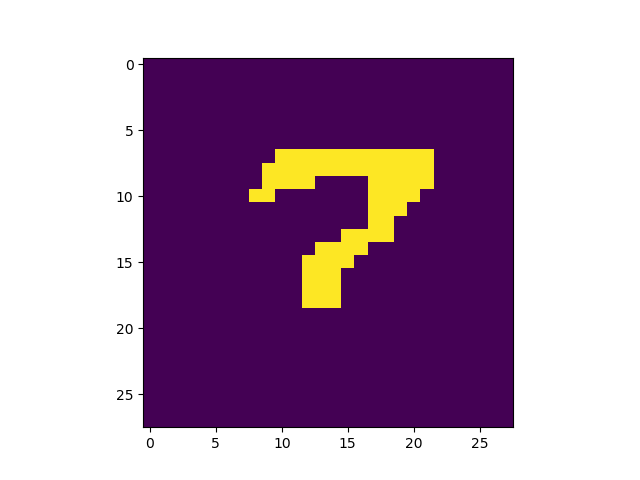
\includegraphics[scale=0.2]{alpha_1_beta_1}
is super smooth, the image looses its meaning.

$\beta=0.6$
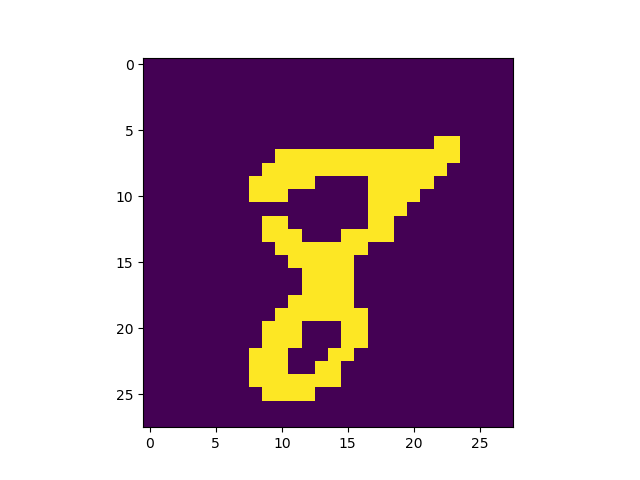
\includegraphics[scale=0.2]{alpha_1_beta_06}
is great.

$\beta=0.5$
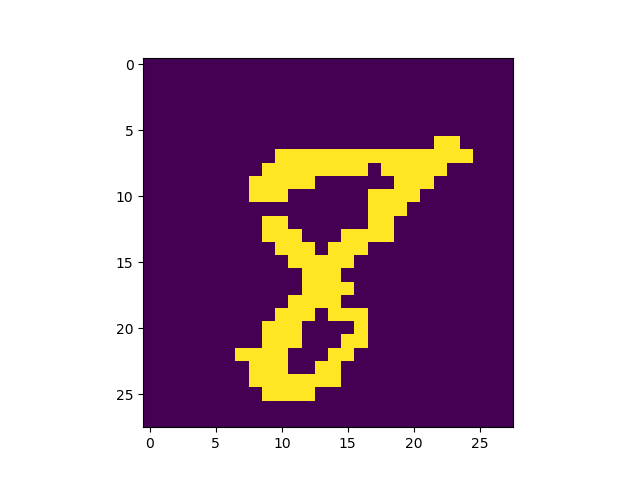
\includegraphics[scale=0.2]{alpha_1_beta_05}
is a bit more loyal to the original image.

$\beta=0.4$
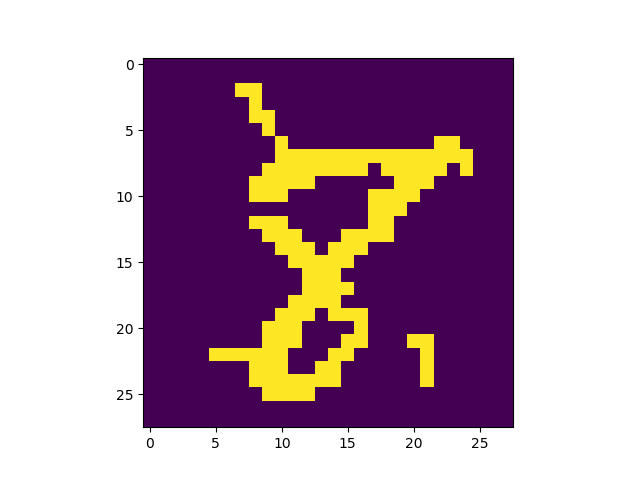
\includegraphics[scale=0.2]{alpha_1_beta_04}
already has the ``noise'' that came with the original drawing, and:

$\beta=0.1$
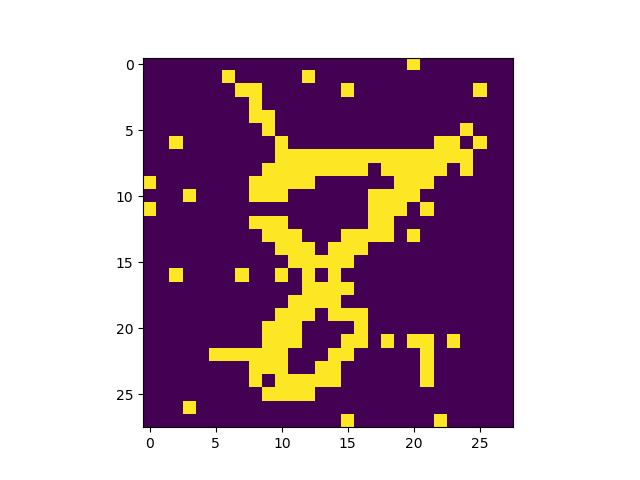
\includegraphics[scale=0.2]{alpha_1_beta_01}
is really identical to the noisy image.

\part*{Q2}
We need to show that the tree-width of a 2D grid graph of size $(m,m)$ is at most $m$. \\*
According to \cite{SEYMOUR199322} if a graph has tree-width of at most $k$ then $k+1$ omniscient cops can catch a robber on G. \\*
On our 2D grid graph , $G$, we will show that we can use a strategy to win the cops and robber game with $m+1$ cops. \\*
Denote the vertices of $G$ by $v_{ij}$. First place $m$ cops on $v_{i1}$ for every $j$ (i.e. the "first column" of $G$). Then for $j=1,...,m$ add a cop to $v_{j2}$ and remove the cop from $v_{j1}$ until all the "second column" vertices are occupied by cops. Continue this process until all vertices $v_{im}$ are occupied by cops. \\*
We can see that at any iteration the cops separate the later columns from the earlier columns so the robber cannot reach earlier columns and will be captured eventually. \\*
QED. 

\part*{Q3}
We now consider the sum-product message update on a tree graph, with the messages updated simultaneously, not recursively. so:
\begin{equation}\label{eq:q3_update}
m_{ij}^{t+1}\left(x_j\right) = \sum_{x_i} \phi_{ij}\left(x_i, x_j\right) \cdot \prod_{k\in N\left(j\right)\setminus i} m_{ki}^t\left(x_i\right)
\end{equation}
We need to prove that at iteration $t=n$ this converges to the true marginals.

We know from class that the recursive algorithm converges to the true marginals, so we will only prove the following fact:
While updating using the simultaneous equations, for an edge $e= i\rightarrow j$, the message computed with the new ("parallel") algorithm converges to the message computed the recursive algorithm, after at most $d$ steps, where $d$ is defined here as the depth of the sub-tree of $i$ as a descendant of $j$.

We will use induction on the depth.
For the base case, with depth $0$, we have to initialize with the uniform distribution, and the result is trivial.

Now we assume for $d_j \le t$, and prove for $d_j = t+1$.
We start with \eqref{eq:q3_update}, and from the assumption we can replace each 
$m_{ki}^t\left(x_i\right)$ with the recursive counterpart $m_{ki}\left(x_i\right)$, to get
\begin{equation*}
m_{ij}^{t+1}\left(x_j\right)=\sum_{x_i} \phi_{ij}\left(x_i, x_j\right) \cdot \prod_{k\in N\left(j\right)\setminus i} m_{ki}\left(x_i\right)
\end{equation*}
\begin{equation*}
m_{ij}^{t+1}\left(x_j\right)=m_{ij}\left(x_j\right)
\end{equation*}
QED.

\part*{Q4}

We consider the pairwise MRF:
$p(x_1,\ldots,x_n) \propto \prod_{ij \in E} \phi_{ij}(x_i,x_j)$.
And define the following ``pseudo-marginals'':
\begin{align}
&\mu_{i}(x_i) &&\propto \prod_{k \in N(i)} m_{ki}(x_i) \\
&\mu_{ij}(x_i, x_j) &&\propto \phi_{ij}(x_i,x_j) \prod_{k \in N(i) \setminus j} m_{ki}(x_i) \prod_{k \in N(j) \setminus i} m_{kj}(x_j)
\end{align}

\section*{a}

We will show that the above pseudo-marginals are indeed correct for tree graphs.
For the next part, we define $ST_j$ to be the sub-tree defined by node $j$ when node $i$ is the root of the tree. $E_{ST_j}$ will be the edges of this sub-tree. Claim:

\begin{equation}
m_{ji}(x_i) = \sum_{(x_k\ |\ k \in ST_j)} \left( \phi_{ij}(x_i,x_j) \prod_{ab \in E_{ST_j}} \phi_{ab}(x_a,x_b) \right)
\end{equation}

We will prove this claim using induction on the depth of $ST_j$. In the base case $j$ is a leaf, $ST_j = {j}$ and $E_{ST_j} = \emptyset$. We then have:

\begin{equation}
m_{ji}(x_i) = \sum_{x_k} \phi_{ij}(x_i,x_j) = \sum_{(x_k\ |\ k \in ST_j)} \left( \phi_{ij}(x_i,x_j) \prod_{ab \in E_{ST_j}} \phi_{ab}(x_a,x_b) \right)
\end{equation}
For the induction step we use the fact that $j$-s children have lower subtrees than $j$,
so the induction hypothesis holds for them:

\begin{align}
m_{ji}(x_i) &= \sum_{x_j} \phi_{ij}(x_i,x_j) \prod_{k \in N(j) \setminus i} m_{kj}(x_j)\\
 &= \sum_{x_j} \phi_{ij}(x_i,x_j) \prod_{k \in N(j) \setminus i}
\left[
	\sum_{(x_l\ |\ l \in ST_k)} \left( \phi_{jk}(x_j,x_k) \prod_{ab \in E_{ST_k}} \phi_{ab}(x_a,x_b) \right) \right]
\end{align}
The outer product is made out of terms, each of which applies to a single subtree.
Each term is a sum of that goes over all possible assignment for this subtree.
Because the different subtrees are disjoint, using the distributivity property we can rearrange the equation and have the an outer sum that goes over all assignments for the union of all subtrees (which is $ST_j$), and for each assignment we have a product of its $\phi$-s.
After rearrangement we are left with:
%\begin{align}
% \sum_{x_j} \sum_{(x_l\ |\ l \in ST_k)} \phi_{ij}(x_i,x_j) \prod_{k \in N(j) \setminus i}
%\left[
%	 \left( \phi_{jk}(x_j,x_k) \prod_{ab \in E_{ST_k}} \phi_{ab}(x_a,x_b) \right) \right]=
%\end{align}
\begin{align}
= \sum_{(x_l\ |\ l \in ST_j)} \left( \phi_{ij}(x_i,x_j) \prod_{ab \in E_{ST_j}} \phi_{ab}(x_a,x_b) \right)
\end{align}
Which proves the claim.
We will now use the claim to substitute it into the definitions of our pseudo-marginals:

\begin{equation}
\mu_{i}(x_i) \propto \prod_{k \in N(i)} m_{ki}(x_i)
= \prod_{k \in N(i)} \left[ \sum_{(x_k\ |\ k \in ST_j)} \left( \phi_{ij}(x_i,x_j) \prod_{ab \in E_{ST_j}} \phi_{ab}(x_a,x_b) \right) \right]
\end{equation}
If we consider $i$ to be the root of the tree,
the summation covers all sub-trees defined by $i$-s children, therefore it covers all nodes except $i$. The inner product covers all edges inside the sub-trees defined by $i$-s children, and the outer product also contains all the edges that connect $i$ to its children, therefore the the product covers all edges in the tree. We can now rewrite the equation as follows:
\begin{equation}
\mu_{i}(x_i) \propto \sum_{\{x_1,\ldots,x_n\}\setminus x_i} \left( \prod_{ab \in E} \phi_{ab}(x_a,x_b) \right) \propto \sum_{\{x_1,\ldots,x_n\}\setminus x_i} p(x_1,\ldots,x_n)
\end{equation}
And this shows that $\mu_i$ is indeed the correct marginal for trees. Similarly, we will substitute into $\mu_{ij}(x_i, x_j)$. The resulting equation is very similar to the previous one, but takes up twice as much space.
Each message $m_{ji}$ transforms into its expanded form, and then we are left with a sum of products. Finally we get:

\begin{equation}
\mu_{ij}(x_i, x_j) \propto \sum_{\{x_1,\ldots,x_n\}\setminus x_i,x_j} \left( \prod_{ab \in E} \phi_{ab}(x_a,x_b) \right) \propto \sum_{\{x_1,\ldots,x_n\}\setminus x_i,x_j} p(x_1,\ldots,x_n)
\end{equation}
Which is the correct marginal. Our pseudo-marginals are indeed the correct marginals for MRF tree graphs.

\section*{b}

We will show that for any graph E (possible non-tree) it holds that:

\begin{equation}
p(x_1,\ldots,x_n) \propto \prod_{i} \mu_{i}(x_i) \prod_{ij \in E} \frac{\mu_{ij}(x_i, x_j)}{\mu_{i}(x_i) \mu_{j}(x_j)}
\end{equation}

We will substitute the definitions of the marginals into the above equation, and then see that all the messages cancel out and only the terms we need are left:

\begin{equation}
\prod_{i} \mu_{i}(x_i) \prod_{ij \in E} \frac{\mu_{ij}(x_i, x_j)}{\mu_{i}(x_i) \mu_{j}(x_j)}
= \prod_{i} \mu_{i}(x_i) \prod_{ij \in E} \frac
{\phi_{ij}(x_i,x_j) \prod_{k \in N(i) \setminus j} m_{ki}(x_i) \prod_{k \in N(j) \setminus i} m_{kj}(x_j)}
{\prod_{k \in N(i)} m_{ki}(x_i) \prod_{k \in N(j)} m_{kj}(x_i)}
\end{equation}
The large fraction has many similarities between its numerator and denominator.
The differences are the $\phi_{ij}$ term in the numerator, and the fact that the product in the
numerator skips over $m_{ji}(x_i)$ and $m_{ij}(x_j)$. After simplification:
\begin{equation}
=\prod_{i} \mu_{i}(x_i) \prod_{ij \in E} \frac
{\phi_{ij}(x_i,x_j)}
{m_{ji}(x_i) m_{ij}(x_j)}
= \\
\left( \prod_{i} \prod_{k \in N(i)} m_{ki}(x_i) \right) \prod_{ij \in E} \frac
{\phi_{ij}(x_i,x_j)}
{m_{ji}(x_i) m_{ij}(x_j)}
\end{equation}
Going over all vertices and then over all inbound edges for each vertex is the same as going over all edges in both directions. Therefore:
\begin{equation}
= \left( \prod_{ij \in E} m_{ji}(x_i) m_{ij}(x_j) \right) \prod_{ij \in E} \frac
{\phi_{ij}(x_i,x_j)}
{m_{ji}(x_i) m_{ij}(x_j)} = \prod_{ij \in E} \phi_{ij}(x_i,x_j) \propto p(x_1,\ldots,x_n)
\end{equation}
QED.

\section*{c}

We will show that at a fixed point of LBP we have: $\sum_{x_j} \mu_{ij}(x_i, x_j) = \mu_i(x_i)$. First, change the marginals into their definitions:

\begin{align}
\sum_{x_j} \mu_{ij}(x_i, x_j) = \sum_{x_j} \phi_{ij}(x_i,x_j) \prod_{k \in N(i) \setminus j} m_{ki}(x_i) \prod_{k \in N(j) \setminus i} m_{kj}(x_j) =\\
= \left(\prod_{k \in N(i) \setminus j} m_{ki}(x_i)\right) \left[\sum_{x_j} \phi_{ij}(x_i,x_j) \prod_{k \in N(j) \setminus i} m_{kj}(x_j)\right]=
\end{align}

The term inside the square brackets is exactly the definition of $m_{ji}$. Because we are in a fixed point of LBP, all values are stable and the messages are consistent with their initial definition (which might not be the case if the algorithm is still running). $m_{ji}$ is up to date with all values in the graph and therefore:
\begin{align}
= \left(\prod_{k \in N(i) \setminus j} m_{ki}(x_i)\right) \left[ m_{ji} \right] = \prod_{k \in N(i)} m_{ki}(x_i) = \mu_i(x_i)
\end{align}

We have shown that at fixed points of LBP: $\sum_{x_j} \mu_{ij}(x_i, x_j) = \mu_i(x_i)$. QED.

\part*{References}
\bibliography{ex2-ref}
\bibliographystyle{plain}


\end{document}